\documentclass[a4paper,12pt]{article}
\usepackage[left=10mm, top=20mm, right=10mm, bottom=20mm, nohead, nofoot]{geometry}
%%% Работа с русским языком
\usepackage{cmap}					% поиск в PDF
\usepackage{mathtext} 				% русские буквы в формулах
\usepackage[T2A]{fontenc}			% кодировка
\usepackage[utf8]{inputenc}			% кодировка исходного текста
\usepackage[english,russian]{babel}	% локализация и переносы
\usepackage{xcolor}
\usepackage{hyperref}
 % Цвета для гиперссылок
\definecolor{linkcolor}{HTML}{799B03} % цвет ссылок
\definecolor{urlcolor}{HTML}{799B03} % цвет гиперссылок

\hypersetup{pdfstartview=FitH,  linkcolor=linkcolor,urlcolor=urlcolor, colorlinks=true}

%%% Дополнительная работа с математикой
\usepackage{amsfonts,amssymb,amsthm,mathtools} % AMS
\usepackage{amsmath}
\usepackage{icomma} % "Умная" запятая: $0,2$ --- число, $0, 2$ --- перечисление

%% Номера формул
%\mathtoolsset{showonlyrefs=true} % Показывать номера только у тех формул, на которые есть \eqref{} в тексте.

%% Шрифты
\usepackage{euscript}	 % Шрифт Евклид
\usepackage{mathrsfs} % Красивый матшрифт

%% Свои команды
\DeclareMathOperator{\sgn}{\mathop{sgn}}

%% Перенос знаков в формулах (по Львовскому)
\newcommand*{\hm}[1]{#1\nobreak\discretionary{}
{\hbox{$\mathsurround=0pt #1$}}{}}
% графика
\usepackage{graphicx}
\graphicspath{{pictures/}}
\DeclareGraphicsExtensions{.pdf,.png,.jpg}
\author{Бурмашев Григорий, БПМИ-208}
\title{Язык SQL, дз  -- 4}
\date{\today}
\begin{document}
\maketitle
\clearpage
\section*{Номер 2}
\begin{center}
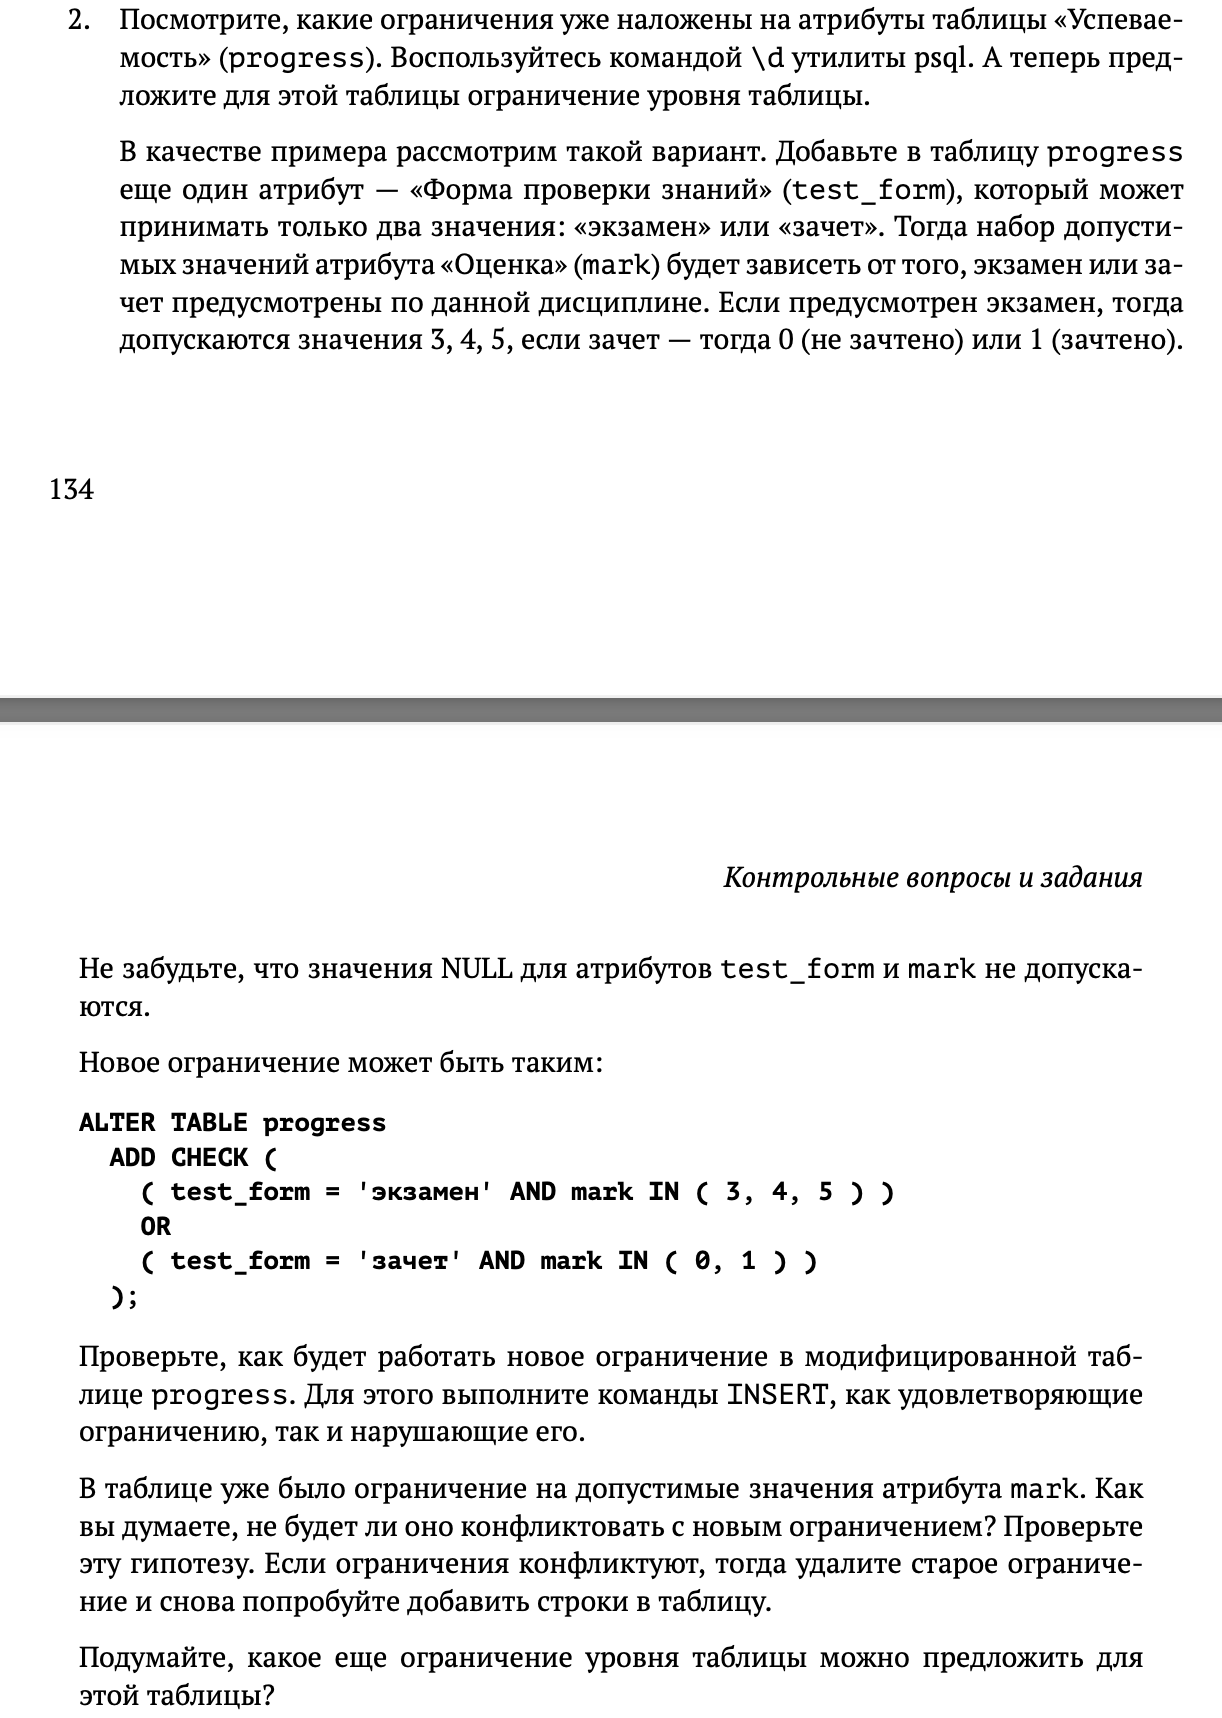
\includegraphics[scale=0.6]{2.png}
\end{center}
\clearpage
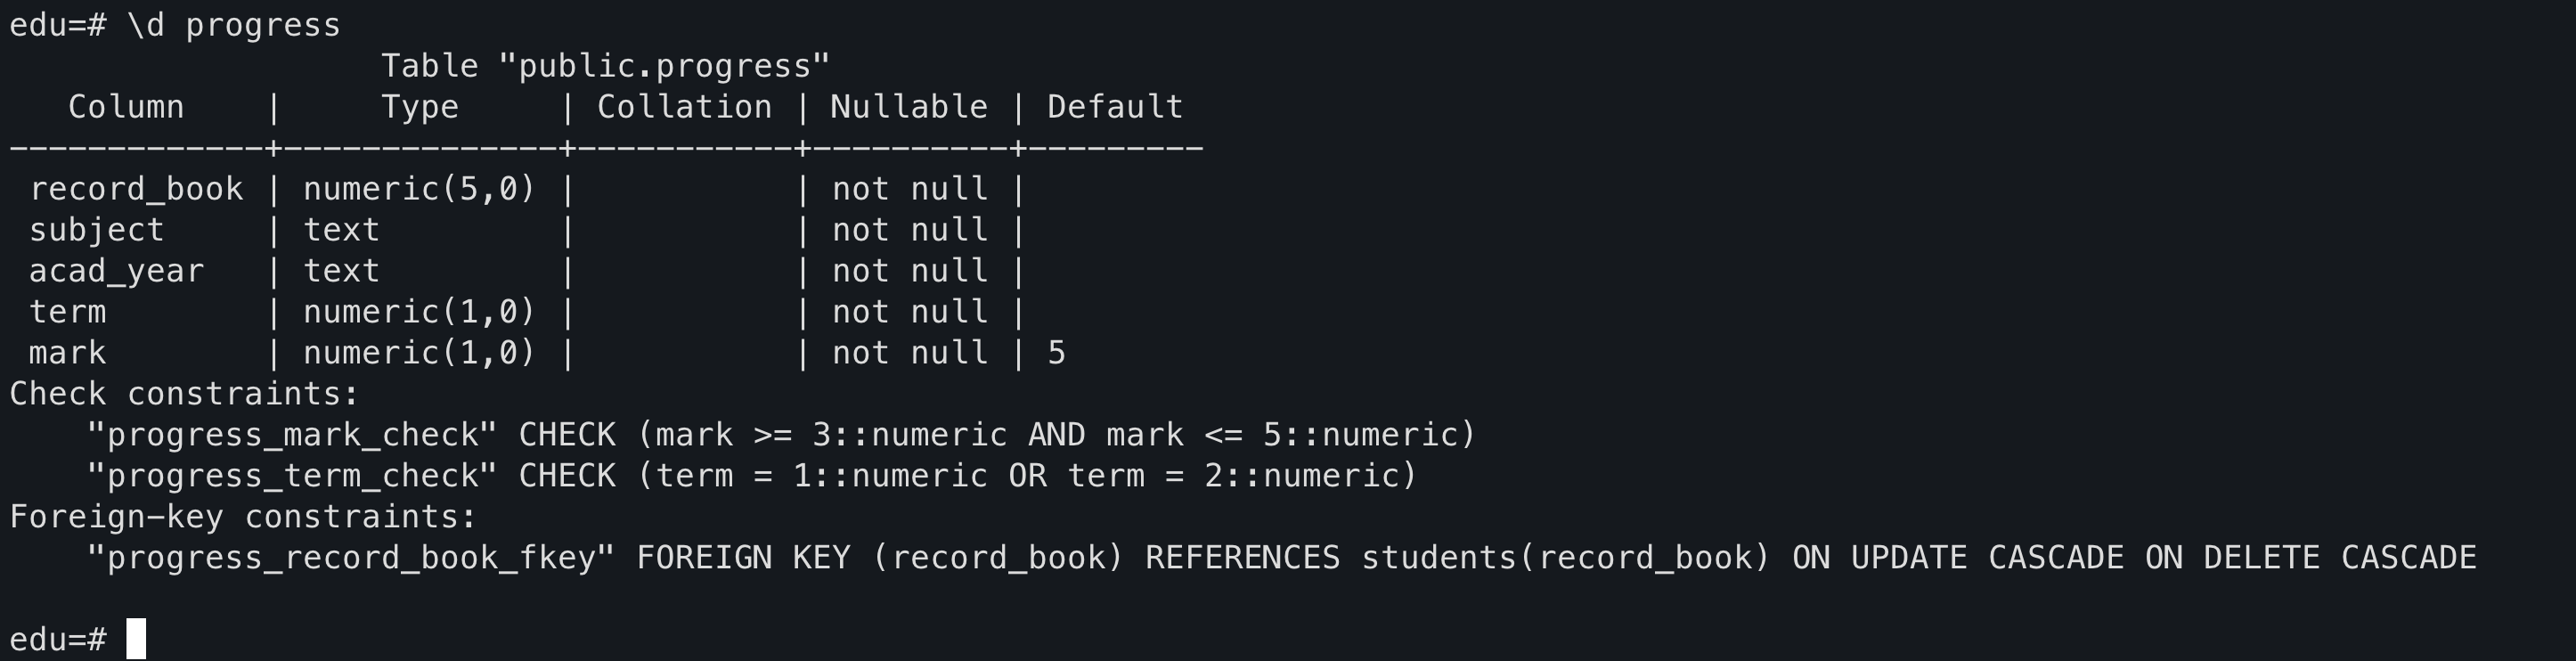
\includegraphics[scale=0.35]{21.png}
\\
Основным атрибутом, на который хочется повесить ограничение является mark, но там ограничение уже есть.
\\\\

\includegraphics[scale=0.5]{22.png}
\\
Добавил новый атрибут test\_form
\\\\
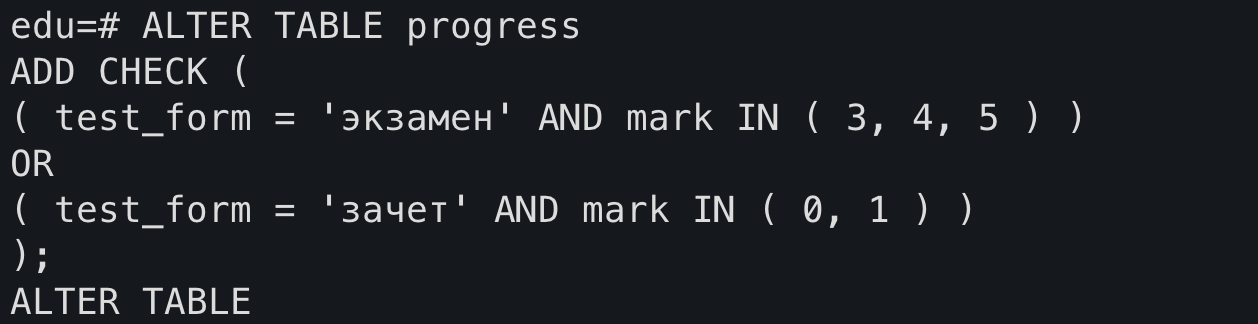
\includegraphics[scale=0.5]{23.png}
\\
Добавил ограничение для test\_form
\\\\
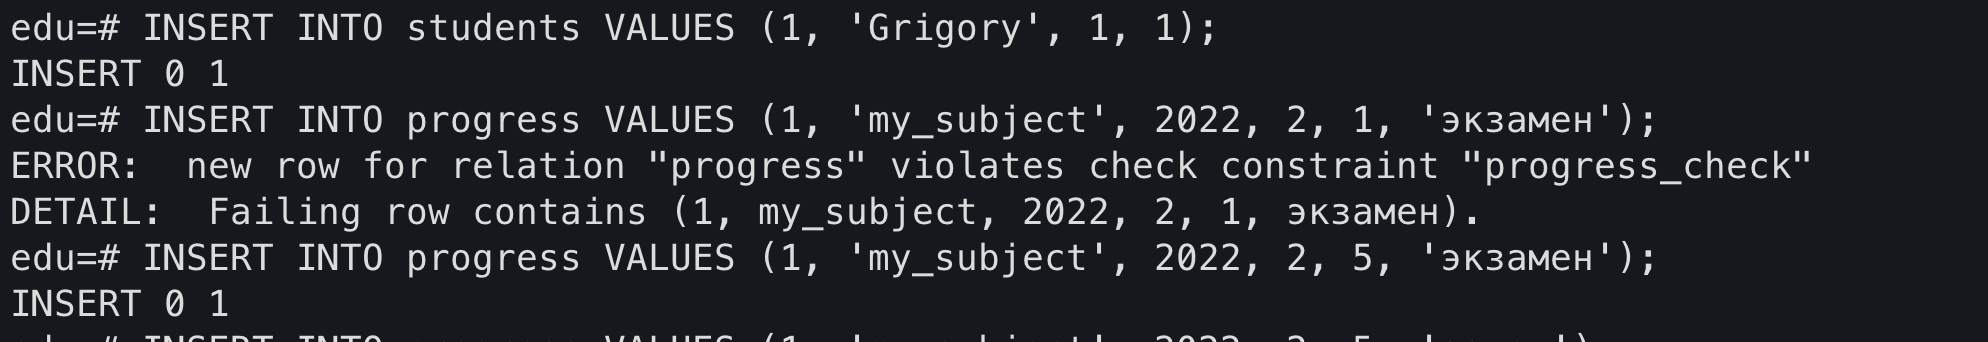
\includegraphics[scale=0.5]{24.png}
\\
Проверяю, что ограничение работает и все хорошо
\\\\

\includegraphics[scale=0.5]{25.png}
\\
Ограничения конфликтуют :(
\\\\
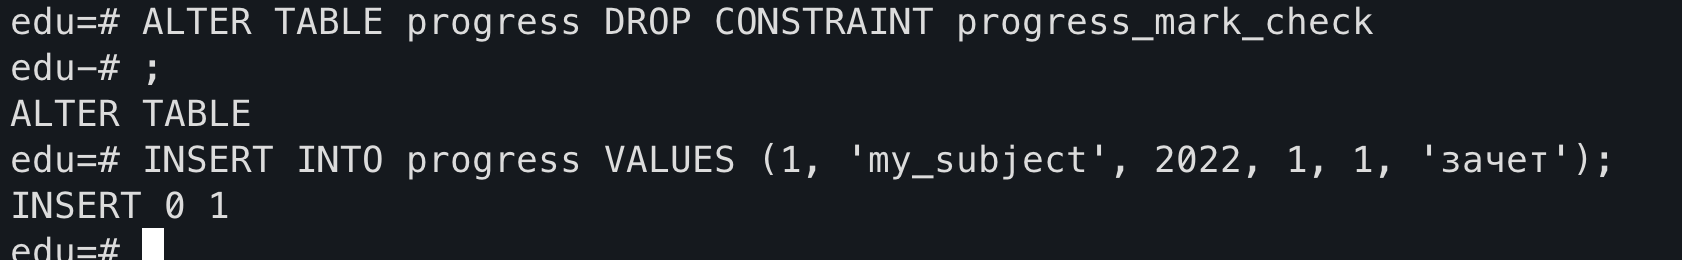
\includegraphics[scale=0.5]{26.png}
\\
Удалил старое ограничение и все пофиксилось.
\\\\\\
Ограничения можно выставить любого характера, например, зафиксировать набор возможных предметов, ограничить возможный год курса и прочее прочее.
\clearpage
\section*{Номер 9}
\begin{center}
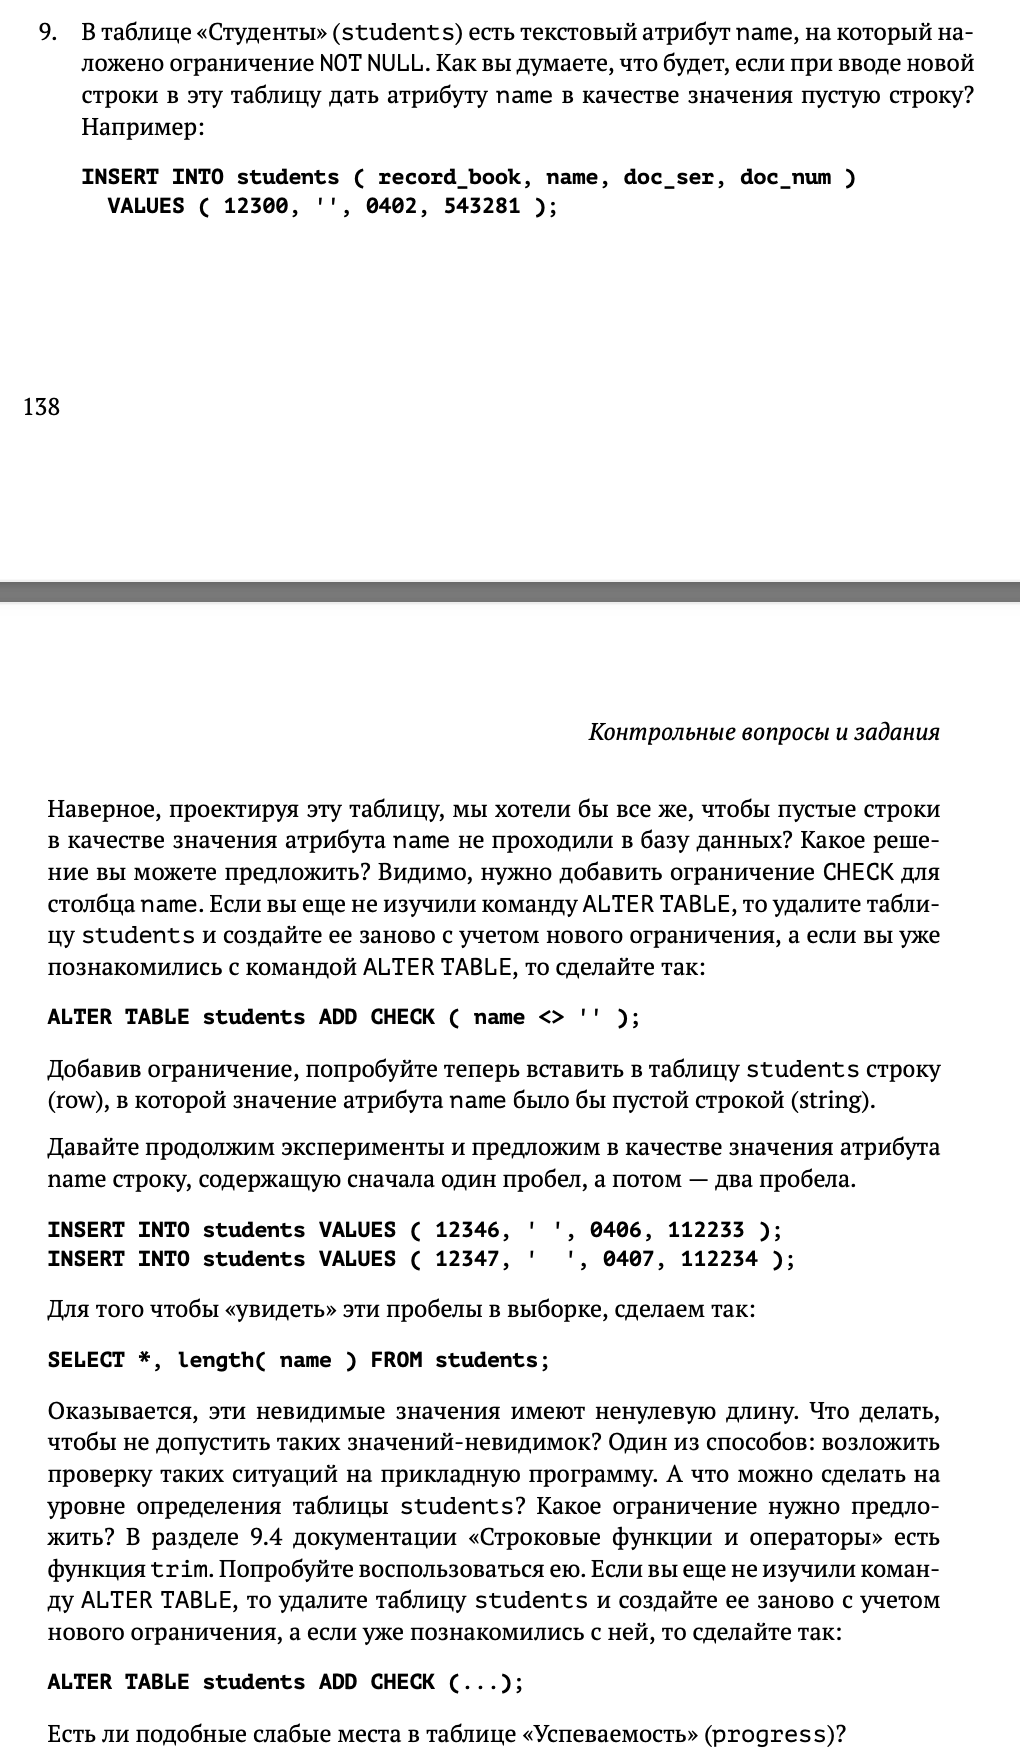
\includegraphics[scale=0.7]{9.png}
\end{center}
\clearpage

\includegraphics[scale=0.5]{91.png}
\\
\text{NULL != ''}, поэтому инсерт происходит успешно
\\\\
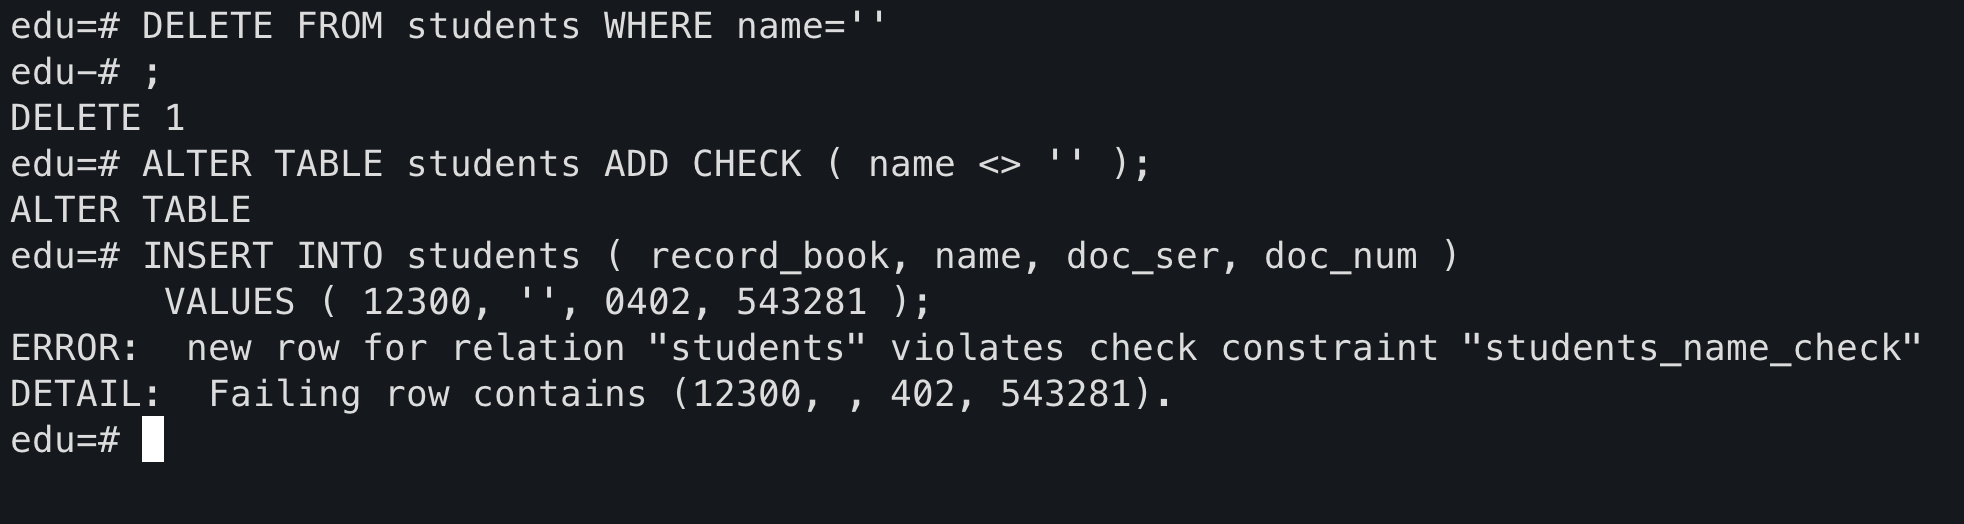
\includegraphics[scale=0.5]{92.png}
\\
Супер, чек начал работать
\\\\
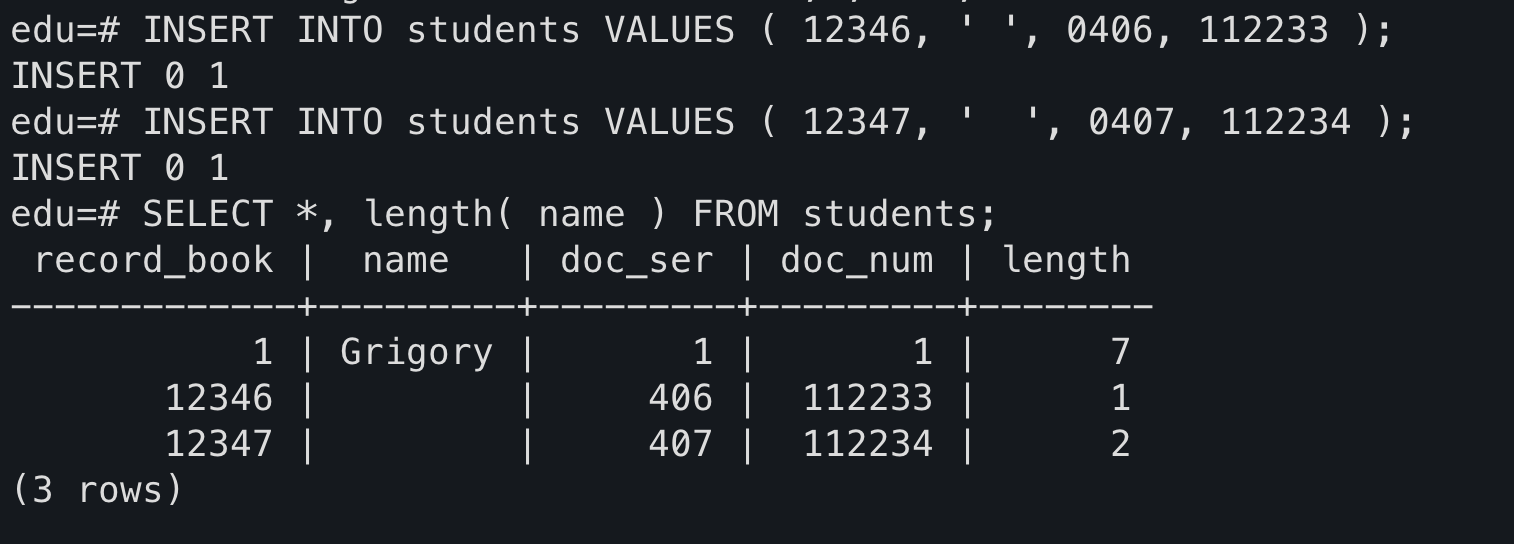
\includegraphics[scale=0.5]{93.png}
\\
Но оказывается работает не так, как ожидалось
\\\\
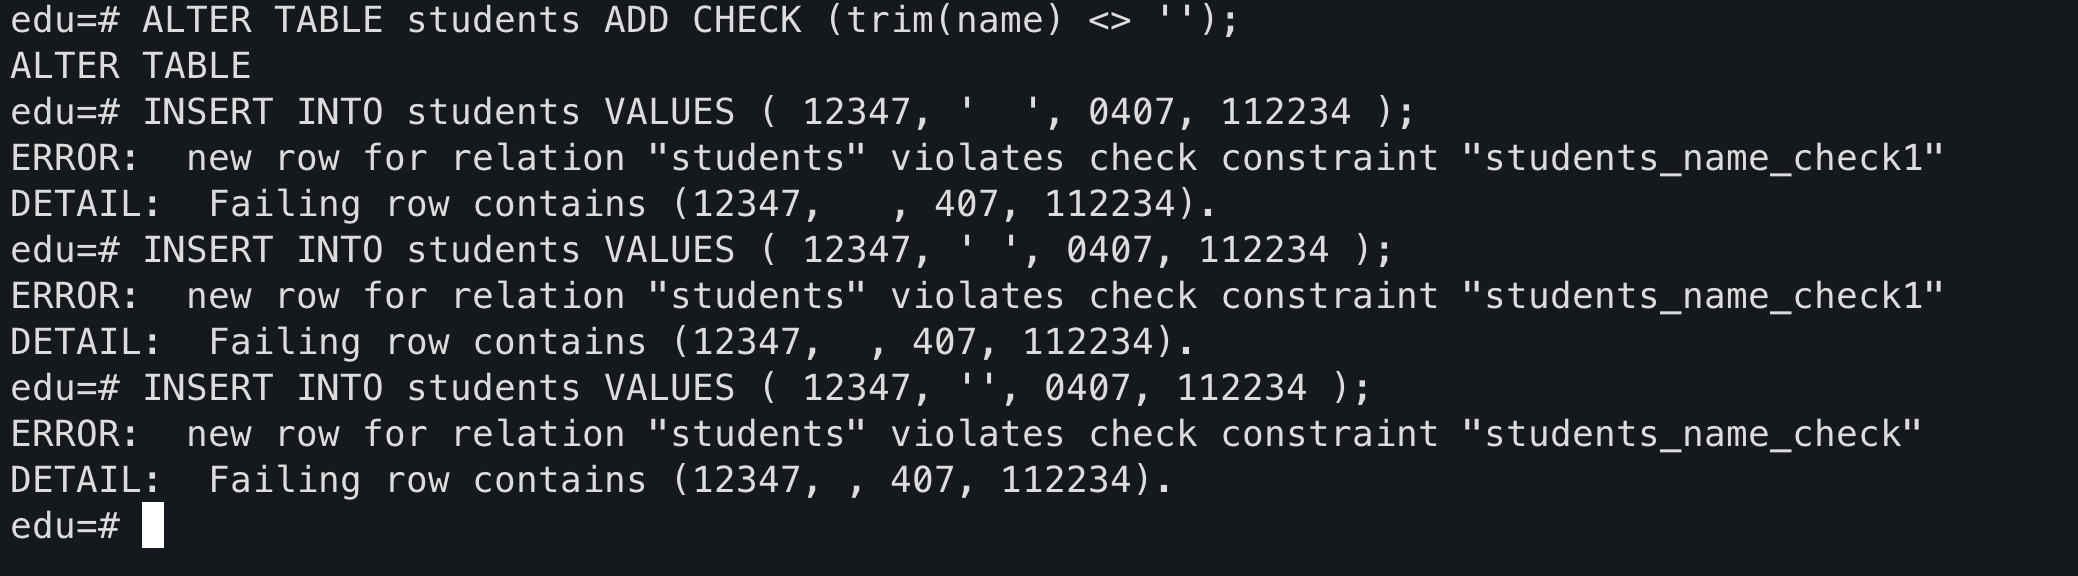
\includegraphics[scale=0.5]{94.png}
\\
Прочитал документацию и пофиксил.
\\\\
В \text{progress} есть слабости у атрибутов \text{subject} и acad\_year (текстовые столбцы)
\clearpage
\section*{Номер 17}
\begin{center}
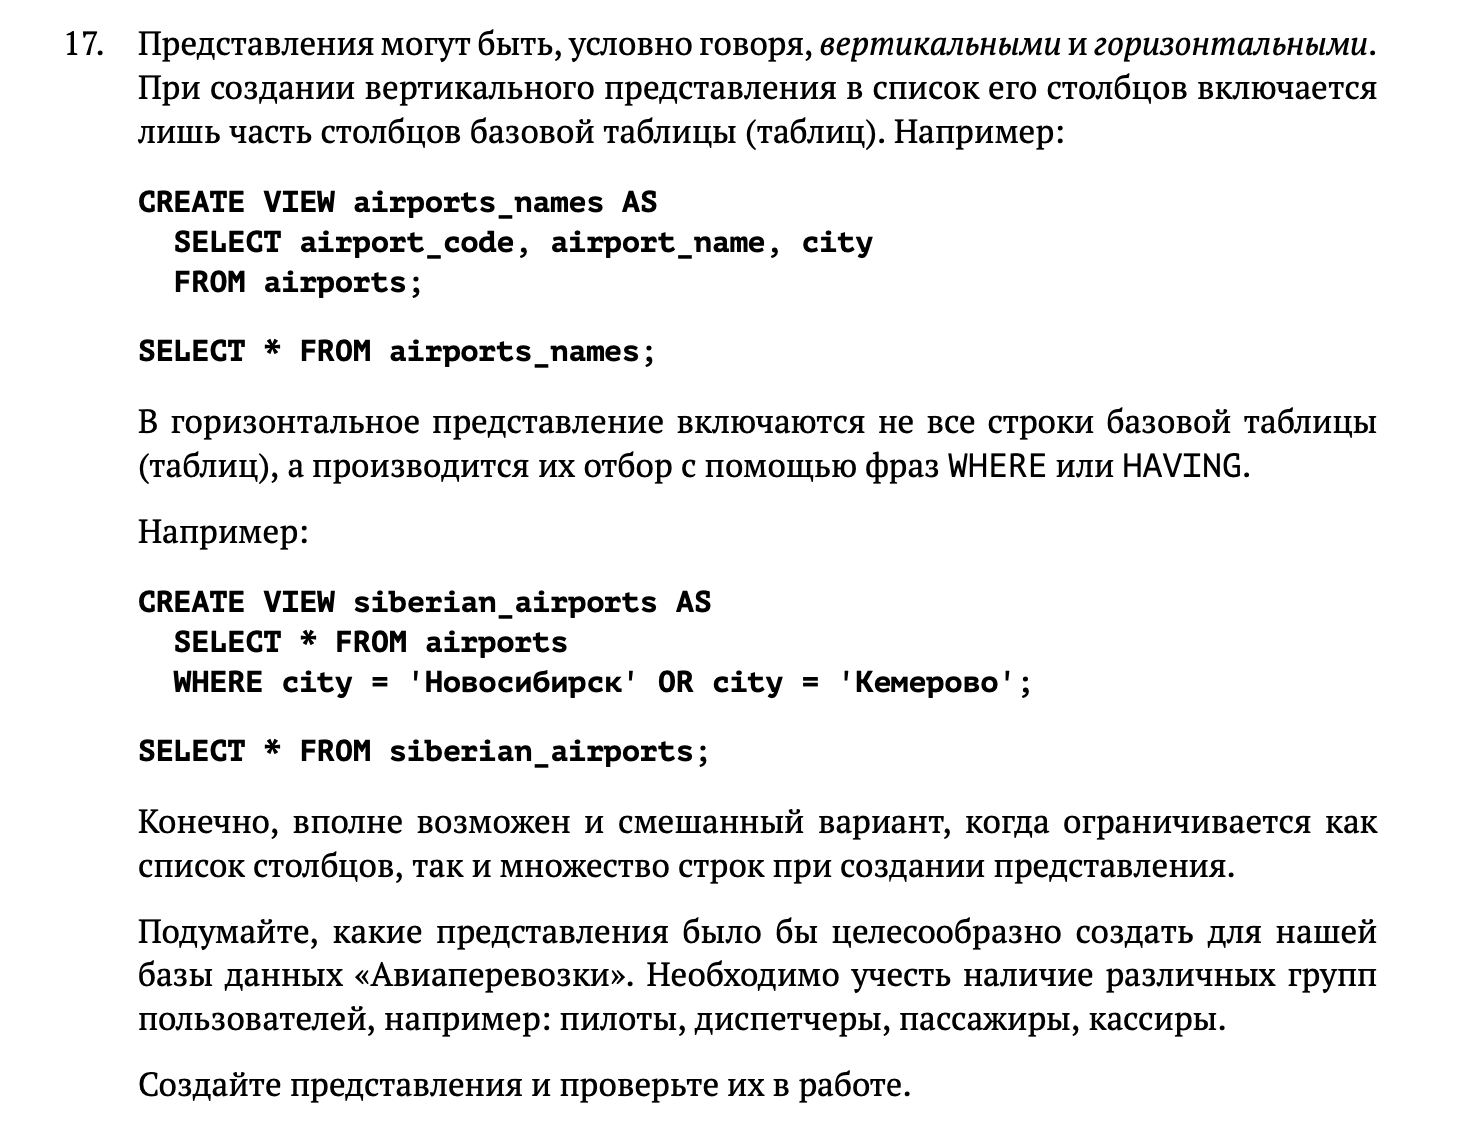
\includegraphics[scale=0.7]{17.png}
\end{center}
\clearpage
Создал представление с указанием координат каждого из аэропортов, это может быть полезно пилотам и диспетчерам
\\\\
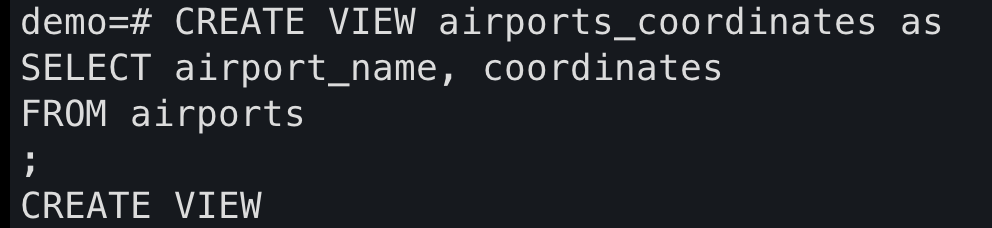
\includegraphics[scale=0.5]{171.png}
\\\\
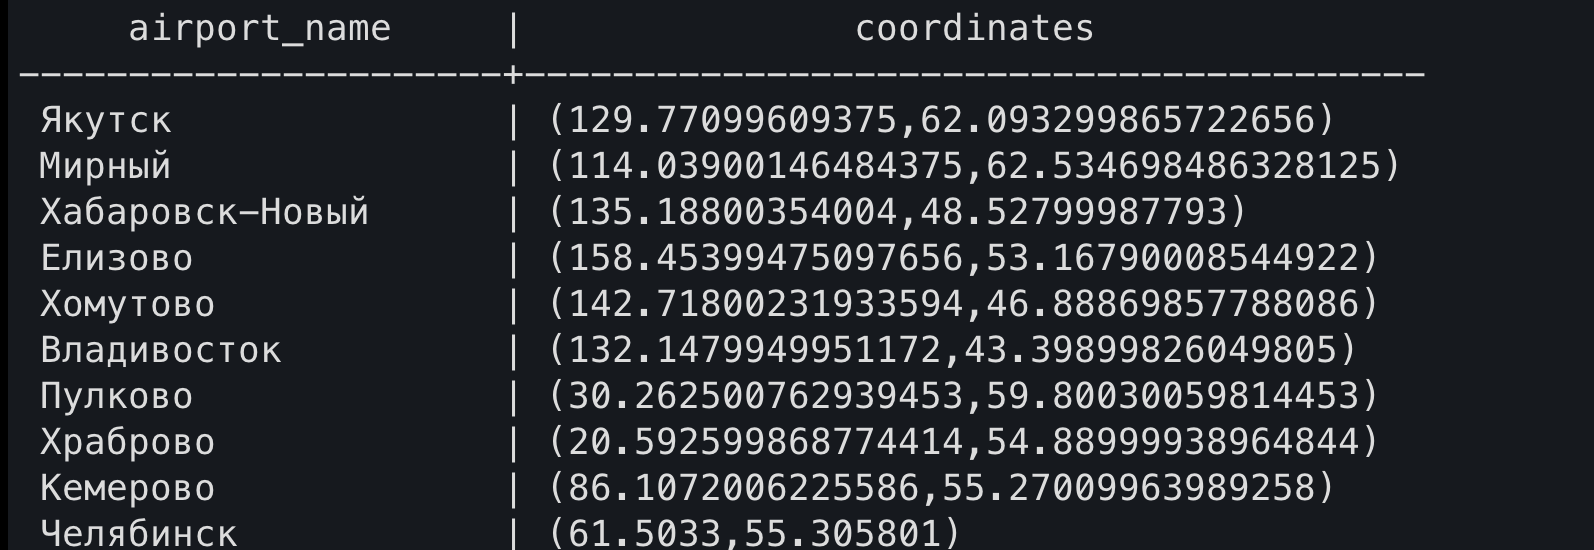
\includegraphics[scale=0.5]{172.png}
\\\\
А еще, например, отображение только Московских аэропортов, это полезно пассажирам -- жителям Москвы
\\\\
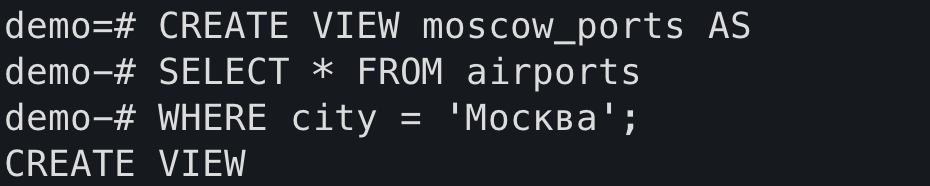
\includegraphics[scale=0.5]{173.png}
\\\\
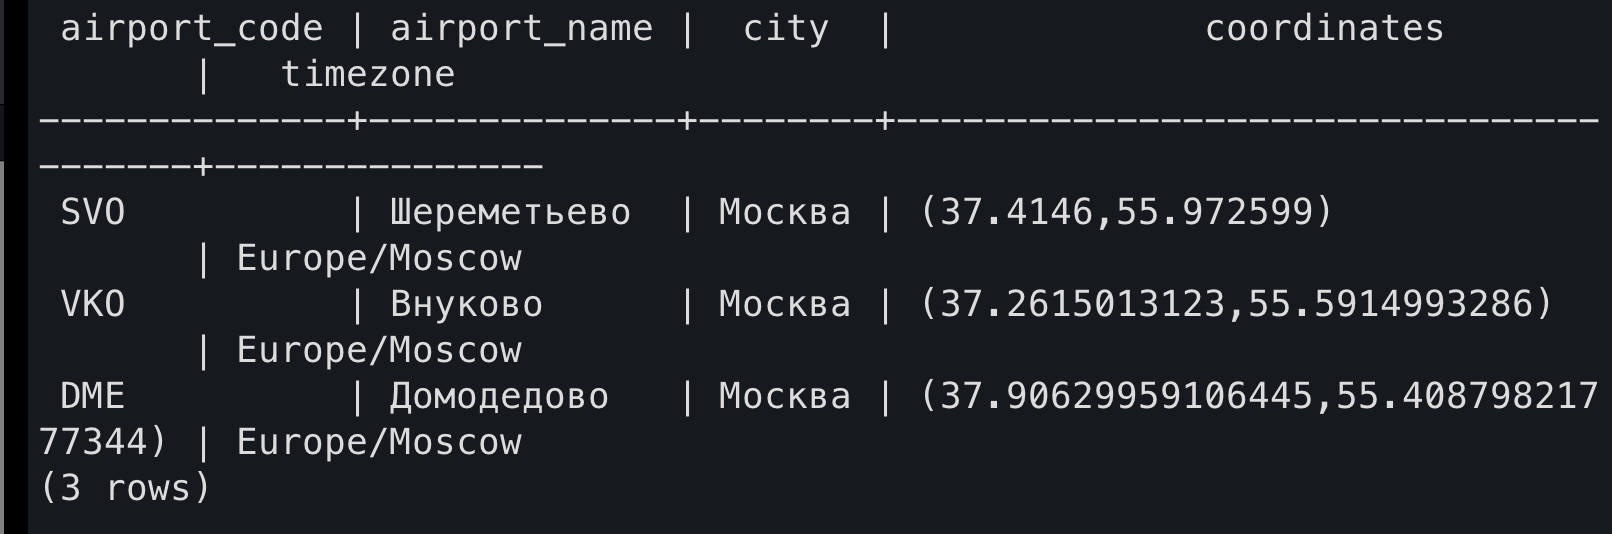
\includegraphics[scale=0.5]{174.png}
\\\\
\clearpage
\section*{Номер 18}
\begin{center}
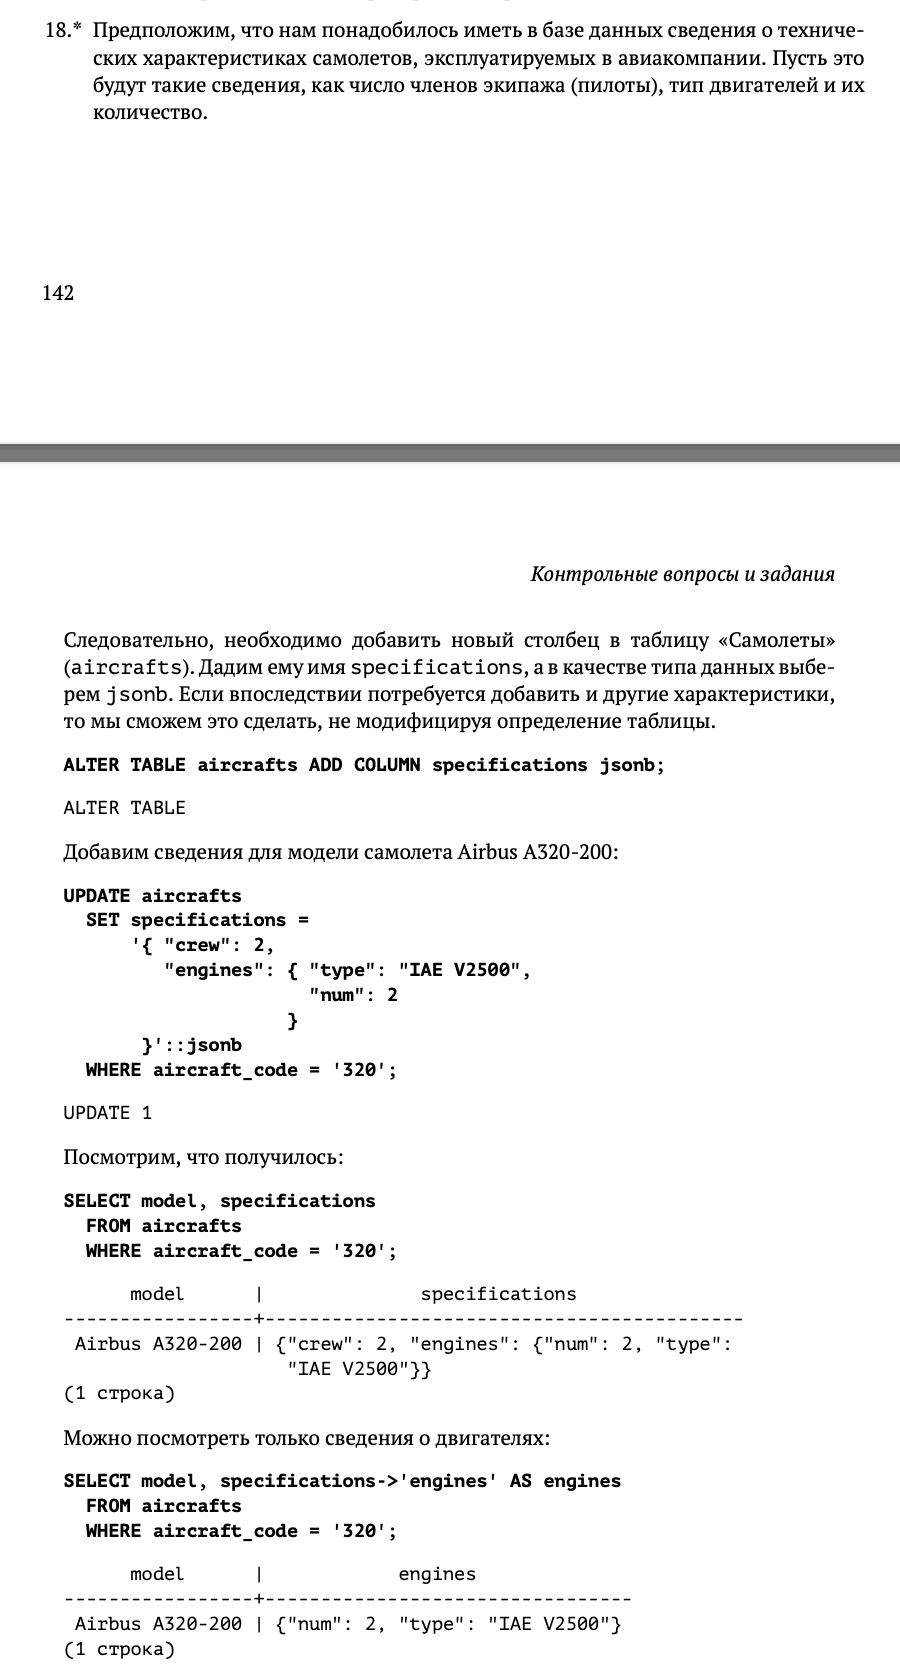
\includegraphics[scale=0.7]{18.png}
\end{center}
\begin{center}
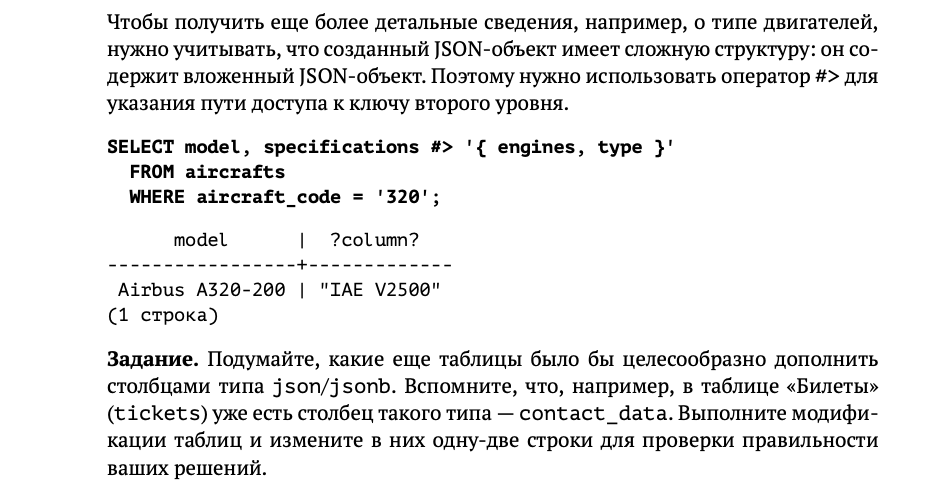
\includegraphics[scale=0.7]{181.png}
\end{center}
\clearpage
Решил создать jsonb в таблице с аэропортами, можно собрать достаточно много информации об аэропортах, число конкретных сотрудников, время/стоимость поездки от аэропорта до города и прочие
\\\\
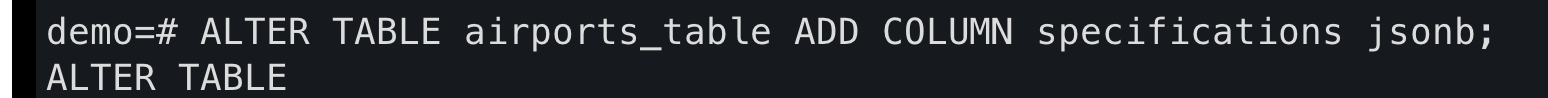
\includegraphics[scale=0.36]{182.png}
\\\\
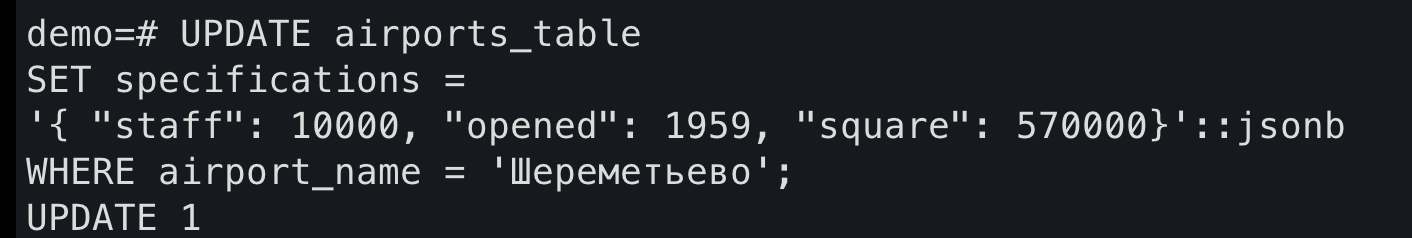
\includegraphics[scale=0.36]{183.png}
\\\\
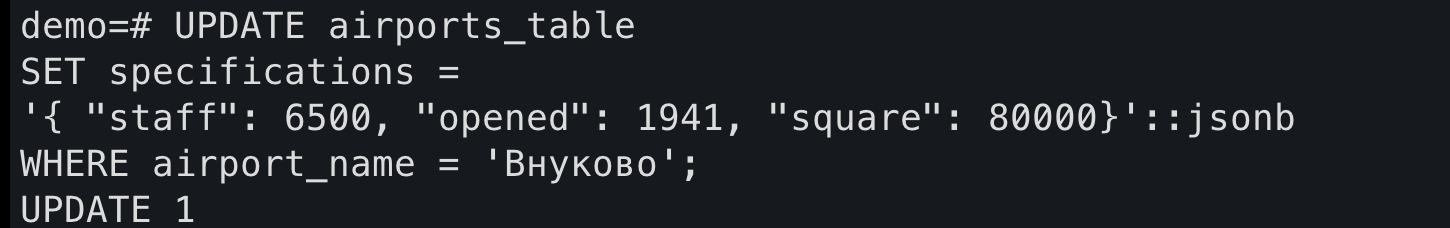
\includegraphics[scale=0.36]{184.png}
\\\\
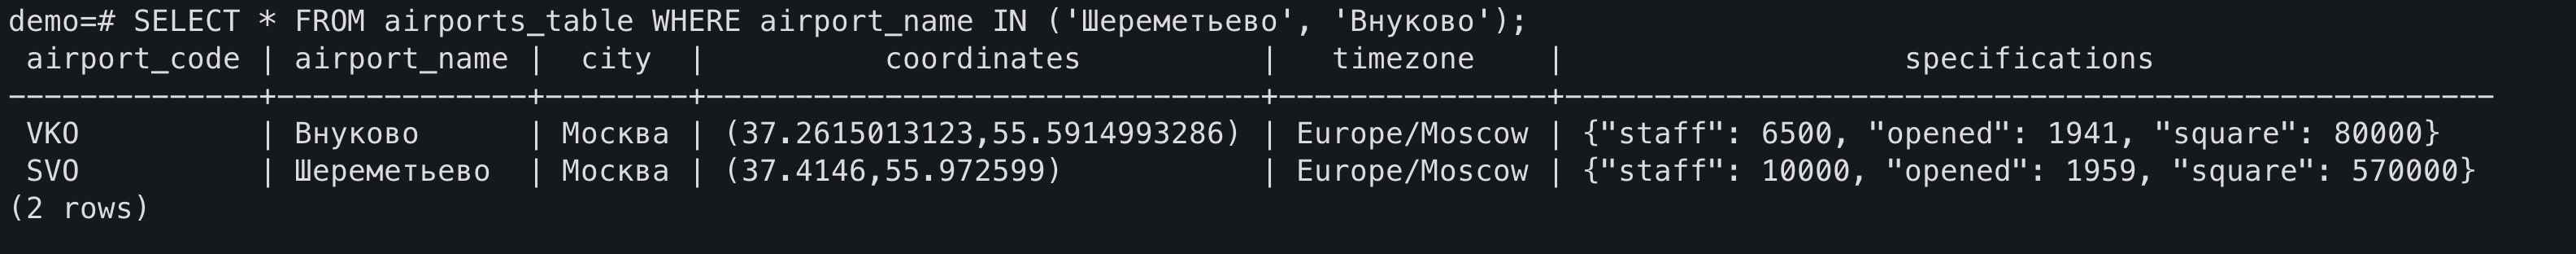
\includegraphics[scale=0.36]{185.png}
\end{document}
